\begin{frame}{PEFT Beyond LoRA}
  \begin{center}
    \Large
    PEFT Beyond LoRA
  \end{center}
\end{frame}

\begin{frame}[t]{The PEFT Family at a Glance}
  \begin{center}
    \scriptsize
    \renewcommand{\arraystretch}{1.35}
    \begin{tabular}{|l|>{\raggedright\arraybackslash}p{5.0cm}|c|c|}
      \hline
      \textbf{Method} & \textbf{What is trained} & \textbf{Trainable} & \textbf{Folds into $W$?} \\
      \hline
      Adapters & Bottleneck MLPs inserted in each block & $\sim$3.6\% & No \\
      Prefix tuning & Key/value prefixes at every layer & $\sim$0.1\% & No \\
      Prompt tuning & A soft prompt at the input layer only & $<$0.01\% & No \\
      LoRA & Low-rank update $\Delta W = BA$ & 0.01--0.2\% & Yes \\
      (IA)$^3$ & Rescaling vectors on $K$, $V$, FFN & $\sim$0.02\% & Yes \\
      DoRA & Magnitude vector plus low-rank direction & $\sim$0.8\% & Yes \\
      \hline
    \end{tabular}
  \end{center}
  \vspace{0.5em}
  {\scriptsize Each percentage is the figure that method's own paper reports, on that paper's own base model --- BERT-base, GPT-2, T5-XXL, T0-3B, LLaMA-7B --- so the column is indicative, not a controlled comparison.}

  \vspace{0.3em}
  {\scriptsize \textbf{Folds into $W$} is the serving question: LoRA, DoRA and (IA)$^3$ are absorbed into the frozen weights after training, so inference costs nothing extra. Adapters and prefixes cannot be.}
\end{frame}

\begin{frame}{Accuracy Against Parameter Budget}
  \begin{figure}
    \centering
    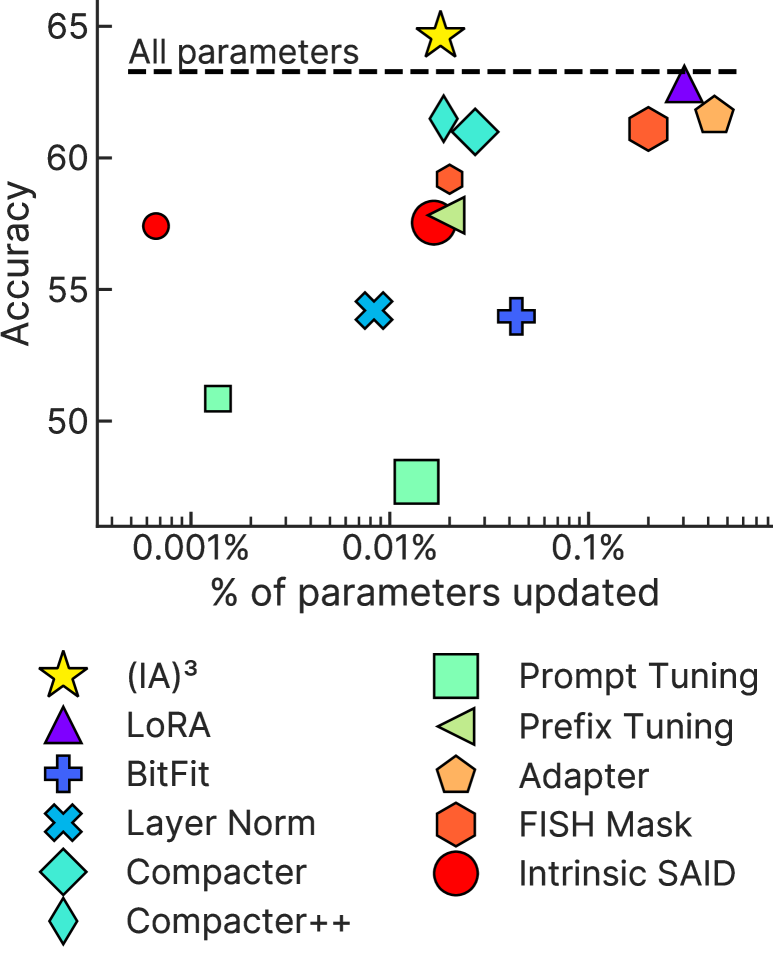
\includegraphics[width=0.42\paperwidth,height=0.62\paperheight,keepaspectratio]{images/llm-rlhf/peft_methods_accuracy_vs_params.png}
    \caption*{\scriptsize Liu et al., ``Few-Shot Parameter-Efficient Fine-Tuning is Better and Cheaper than In-Context Learning,'' \href{https://arxiv.org/abs/2205.05638v2}{arXiv:2205.05638v2}, Figure~2. PEFT methods applied to T0-3B; the dashed line is full fine-tuning.}
  \end{figure}
\end{frame}

\begin{frame}[t]{Soft Prompts: Prefix and Prompt Tuning}
  \begin{itemize}\itemsep0.5em
    \item[\textcolor{red}{$\blacktriangleright$}] \textbf{Key idea:} Leave every weight frozen and learn the \emph{input} instead --- a short sequence of continuous vectors that behave like tokens but never map to real words.
    \item[\textcolor{red}{$\blacktriangleright$}] \textbf{Prefix tuning} (Li \& Liang, 2021) prepends trainable key/value vectors at \emph{every} transformer layer, so later tokens attend to them as virtual tokens. About 0.1\% of parameters. Optimising the prefix directly proved unstable, so it is reparameterised through a small MLP during training and discarded afterwards.
    \item[\textcolor{red}{$\blacktriangleright$}] \textbf{Prompt tuning} (Lester et al., 2021) simplifies this to the \emph{input embedding layer only}, with no reparameterisation. A 100-token prompt for T5-XXL is 409{,}600 parameters, roughly 0.004\% of the model.
    \item[\textcolor{red}{$\blacktriangleright$}] Neither method touches a single pre-trained weight, so one frozen copy of the model can serve every task you have ever tuned.
  \end{itemize}
\end{frame}

\begin{frame}[t]{Soft Prompts: Where They Win}
  \begin{itemize}\itemsep0.6em
    \item[\textcolor{red}{$\blacktriangleright$}] \textbf{Storage.} A thousand tenants means a thousand prompt files of a few hundred kilobytes, on one shared model --- not a thousand adapter checkpoints.
    \item[\textcolor{red}{$\blacktriangleright$}] \textbf{Small data.} Prefix tuning beats full fine-tuning at 50--500 training examples ($+2.9$ BLEU on average) and extrapolates better to unseen topics.
    \item[\textcolor{red}{$\blacktriangleright$}] \textbf{Domain shift.} Freezing the general-purpose weights limits overfitting: prompt tuning trained on SQuAD and evaluated zero-shot on TextbookQA beat full model tuning by 12.5 F1.
  \end{itemize}
\end{frame}

\begin{frame}[t]{Soft Prompts: Where They Lag}
  \begin{itemize}\itemsep0.6em
    \item[\textcolor{red}{$\blacktriangleright$}] \textbf{Scale dependence.} Prompt tuning only reaches parity with full fine-tuning once the frozen model is large --- Lester et al.\ show the gap closing at T5-XXL (11B) and widening steadily below it.
    \item[\textcolor{red}{$\blacktriangleright$}] \textbf{Context budget.} A 100-token prefix is 100 tokens the user no longer has, on every request forever.
    \item[\textcolor{red}{$\blacktriangleright$}] \textbf{No fold-in.} The prefix must be re-inserted at inference, so it is a permanent change to the serving path rather than a one-off weight edit.
  \end{itemize}
\end{frame}

\begin{frame}[t]{Adapters and (IA)$^3$}
  \begin{itemize}\itemsep0.35em
    \item[\textcolor{red}{$\blacktriangleright$}] \textbf{Adapters} (Houlsby et al., 2019) insert a bottleneck module twice per block --- after the attention projection and after the feed-forward layers. Each projects $d \to m$, applies a nonlinearity, projects back $m \to d$, and adds a skip connection: $2md + d + m$ parameters with $m \ll d$, initialised near zero so the module starts as an approximate identity.
      \begin{itemize}
        \item 3.6\% of parameters per task, within 0.4\% of full fine-tuning on GLUE --- but real depth added to every forward pass.
      \end{itemize}
    \item[\textcolor{red}{$\blacktriangleright$}] \textbf{(IA)$^3$} (Liu et al., 2022) adds no modules and trains no weights. It rescales three sets of \emph{activations} element-wise with learned vectors $l_k$, $l_v$, $l_{\mathrm{ff}}$:
      \[
        \mathrm{softmax}\!\left(\frac{Q\,(l_k \odot K^{\top})}{\sqrt{d_k}}\right)(l_v \odot V),
        \qquad
        \big(l_{\mathrm{ff}} \odot \gamma(W_1 x)\big)\,W_2
      \]
      540K parameters for T0-3B ($0.018\%$). Since $l \odot Wx = (l \odot W)x$, the vectors fold permanently into the weights; and because the rescaling is on activations, one batch can serve several tasks at once.
  \end{itemize}
\end{frame}

\begin{frame}[t]{DoRA: Magnitude and Direction}
  \begin{itemize}\itemsep0.4em
    \item[\textcolor{red}{$\blacktriangleright$}] \textbf{Observation:} split a weight matrix into how long each column is and where it points, and full fine-tuning moves the two \emph{independently}, while LoRA ties them together.
    \item[\textcolor{red}{$\blacktriangleright$}] \textbf{DoRA} (Liu et al., 2024) makes that split explicit before adapting:
      \[
        W = m\,\frac{V}{\lVert V \rVert_c},
        \qquad m \in \mathbb{R}^{1 \times k},\quad V \in \mathbb{R}^{d \times k}
      \]
      where $\lVert \cdot \rVert_c$ is the vector norm taken down each column: $m$ holds one magnitude per column, $V$ holds the directions.
    \item[\textcolor{red}{$\blacktriangleright$}] Initialise $m = \lVert W_0 \rVert_c$ and $V = W_0$, then adapt \emph{only the direction} with LoRA while training the magnitude vector directly:
      \[
        W' = m\,\frac{W_0 + BA}{\lVert W_0 + BA \rVert_c}
      \]
      $m$, $B$ and $A$ are trained; $W_0$ stays frozen, and the whole thing folds back into one matrix for serving.
  \end{itemize}
\end{frame}

\begin{frame}{DoRA: Magnitude and Direction}
  \begin{figure}
    \centering
    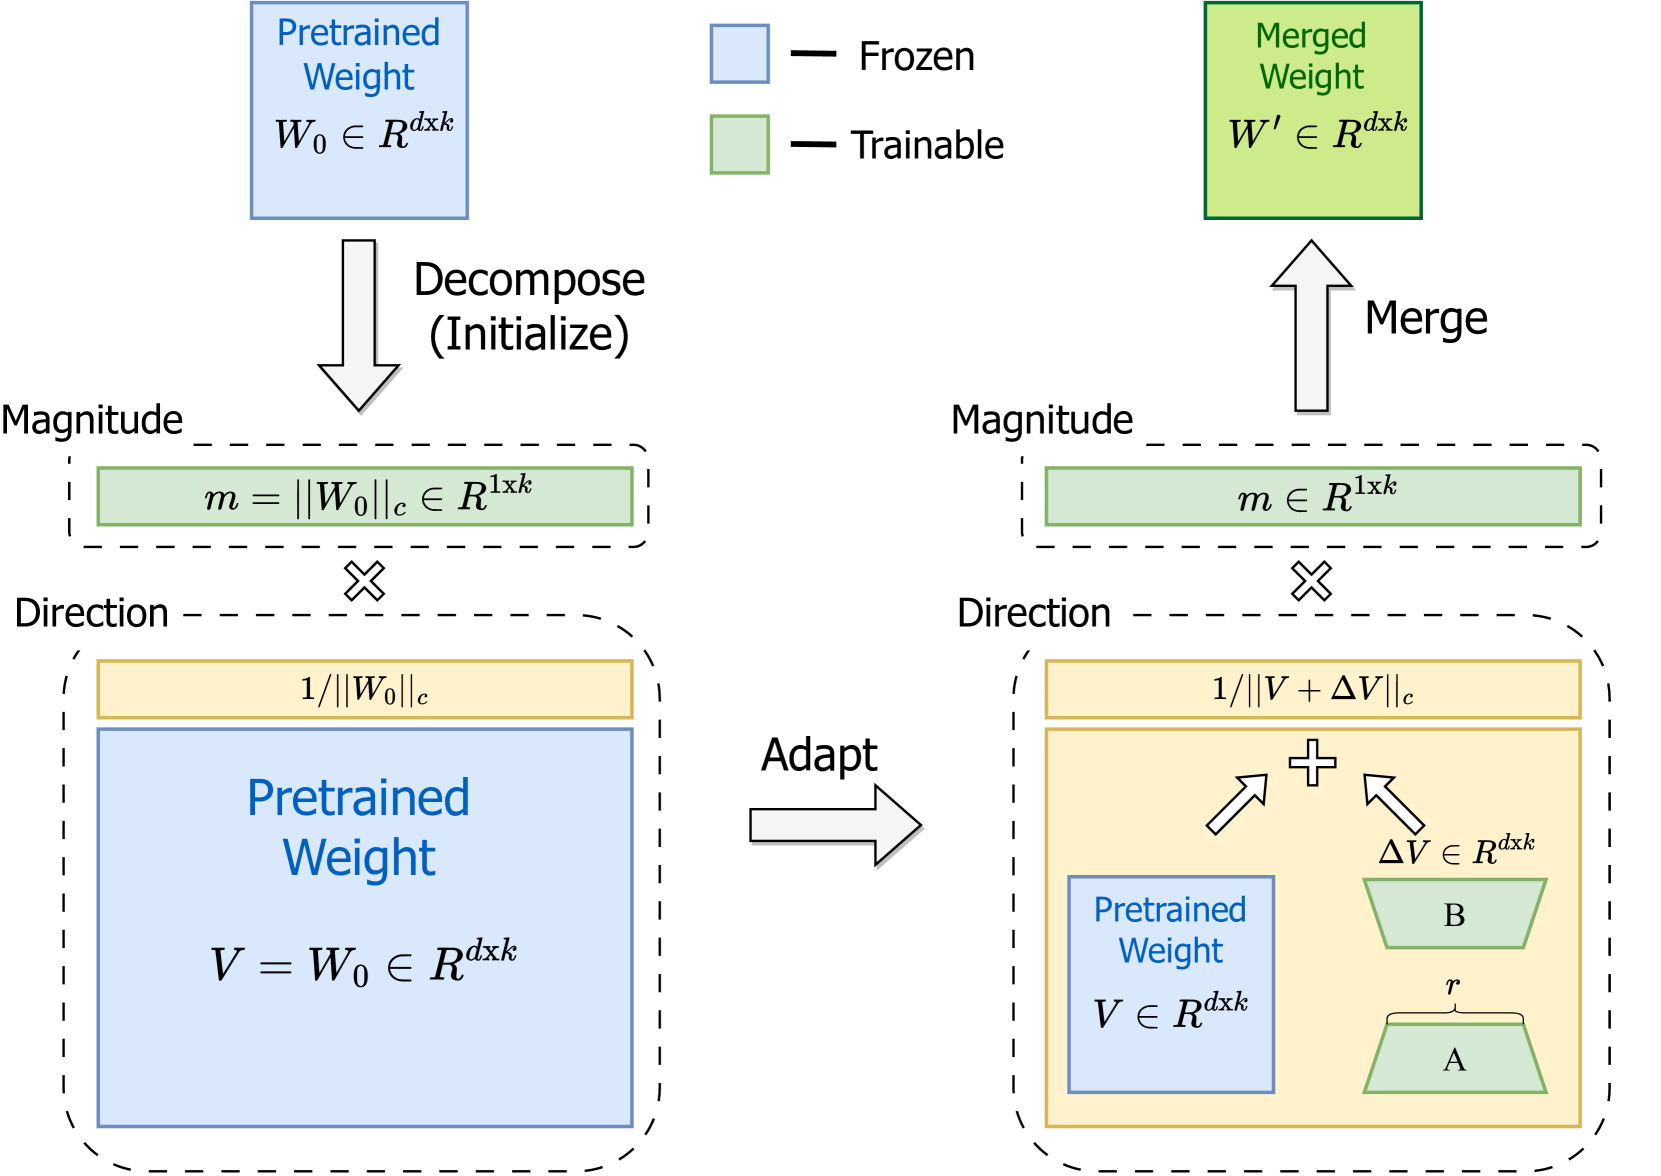
\includegraphics[width=0.52\paperwidth,height=0.62\paperheight,keepaspectratio]{images/llm-rlhf/peft_dora_decomposition.png}
    \caption*{\scriptsize Liu et al., ``DoRA: Weight-Decomposed Low-Rank Adaptation,'' \href{https://arxiv.org/abs/2402.09353v6}{arXiv:2402.09353v6}, Figure~1.}
  \end{figure}
\end{frame}

\begin{frame}[t]{Choosing a PEFT Method}
  \begin{itemize}\itemsep0.4em
    \item[\textcolor{red}{$\blacktriangleright$}] \textbf{Default to LoRA or DoRA.} Good accuracy, no inference overhead, and every serving stack supports them. The extra magnitude vector costs $k$ numbers per matrix, so DoRA sits at the same trainable fraction as LoRA (about 0.8\% at 7B) and pays off most at low rank: on commonsense reasoning it reaches 78.4 vs LoRA's 74.7 on LLaMA-7B, and 85.2 vs 80.8 on LLaMA3-8B.
    \item[\textcolor{red}{$\blacktriangleright$}] \textbf{Many tenants, one model?} Soft prompts or (IA)$^3$. Per-tenant state drops to kilobytes, and (IA)$^3$ additionally lets one batch serve several tenants.
    \item[\textcolor{red}{$\blacktriangleright$}] \textbf{Tens to hundreds of examples?} Soft prompts and (IA)$^3$ hold up better than methods with more capacity to overfit.
    \item[\textcolor{red}{$\blacktriangleright$}] \textbf{A genuinely new capability, not a new style?} No PEFT method will get you there --- that is a full fine-tune or continued pre-training question.
    \item[\textcolor{red}{$\blacktriangleright$}] \textbf{Adapters} are now mostly of historical interest for LLMs: they cost latency the fold-in methods do not, for no accuracy advantage.
  \end{itemize}
\end{frame}
